\documentclass[5p,times,twocolumn]{elsarticle}

\usepackage{graphicx}
\graphicspath{{Figures/}}%% upload the Figures/ folder (not its contents into the project root)
\usepackage{amsmath,amssymb}
\usepackage{booktabs}
\usepackage[hyphens]{url}
\usepackage{hyperref}

\journal{SoftwareX}

\begin{document}

\begin{frontmatter}

\title{Neuro-DT Dashboard: a Streamlit-based clinical interface for Brain Digital Twin Alzheimer's Disease risk prediction, explainability, and intervention simulation}

\author[aastmt]{Seif Hendawy\corref{cor1}}
\ead{S.Aboelha33814@student.aast.edu}

\author[aastmt]{Fahima Maghraby}
\ead{Fahima@aast.edu}

\author[aastmt]{Ahmed Salem}
\ead{a.salem@aast.edu}

\cortext[cor1]{Corresponding author.}
\address[aastmt]{Computer Science, Arab Academy for Science, Technology and Maritime Transport (AASTMT), Sheraton, Cairo, Egypt}

\begin{abstract}
Clinicians evaluating disease-modifying therapies for Alzheimer's Disease (AD) need more than a diagnostic label: they need a confidence estimate, an explanation of which anatomical and clinical features drove it, and a forward-looking view of how a patient's risk trajectory might change under different treatment scenarios, all without having to run research code. We present the Neuro-DT Dashboard, a Streamlit-based clinical interface that wraps a trained hybrid 3D CNN-Transformer classifier and an empirically estimated, APOE4-stratified Markov progression model into a single interactive application, containerized and deployed to Azure App Service. The dashboard integrates live SHAP and Grad-CAM explainability, a Monte Carlo trajectory simulator covering genetic-risk and pharmacological-intervention scenarios (Lecanemab, Donanemab), a 5-year dementia risk-factor breakdown, and an AI-generated lifestyle-recommendation panel, alongside the diagnostic prediction and model-information views. The deployed application was validated against a genuine held-out patient record, correctly predicting the true diagnosis with near-full confidence and reproducing hand-computed risk-trajectory values independently. Three integration-stage defects, a checkpoint-loading incompatibility, a label-mapping mismatch between model checkpoint generations, and a silent-failure mode for patients with no cached MRI scan, were identified and resolved prior to release, and are documented here as reusable lessons for deploying similar research models into clinical-facing interfaces.
\end{abstract}

\begin{keyword}
Clinical dashboard \sep Brain Digital Twin \sep Alzheimer's Disease \sep Streamlit \sep Explainable AI \sep Markov Chain simulation \sep Clinical decision support
\end{keyword}

\end{frontmatter}

\begin{table*}[t]
\centering
\caption{Code metadata}
\label{tab:metadata}
\begin{tabular}{@{}p{0.04\textwidth}p{0.30\textwidth}p{0.58\textwidth}@{}}
\toprule
Nr & Code metadata description & Metadata \\
\midrule
C1 & Current code version & v1.0 \\
C2 & Permanent link to code/repository used for this code version & \url{https://github.com/Hendawyy/neuro-dt-dashboard} \\
C3 & Permanent link to reproducible capsule & \texttt{[ADD IF ARCHIVED, E.G. A ZENODO DOI]} \\
C4 & Legal code license & MIT \\
C5 & Code versioning system used & Git \\
C6 & Software code languages, tools and services used & Python, Streamlit, PyTorch, Docker, Azure App Service \\
C7 & Compilation requirements, operating environments and dependencies & Python 3.10+; PyTorch, Streamlit, scikit-learn, SHAP, pandas, NumPy; Linux container deployed via Docker to Azure App Service \\
C8 & If available, link to developer documentation/manual & \url{https://github.com/Hendawyy/neuro-dt-dashboard#readme} \\
C9 & Support email for questions & \href{mailto:S.Aboelha33814@student.aast.edu}{S.Aboelha33814@student.aast.edu} \\
\bottomrule
\end{tabular}
\end{table*}

\section{Motivation and significance}\label{sec1}

Disease-modifying therapies (DMTs) for Alzheimer's Disease, such as Lecanemab \cite{bib_lecanemab} and Donanemab, have shifted the clinical question from ``does this patient have AD'' to ``how will this specific patient's trajectory change under a specific intervention, and how confident should that forecast be.'' A companion research effort developed the Brain Digital Twin (BDT), a hybrid 3D DenseNet-121 convolutional and Transformer classifier for multimodal Alzheimer's diagnosis, combined with an empirically estimated, APOE4-stratified Markov Chain progression model that simulates patient-specific trajectories under genetic-risk and pharmacological-intervention scenarios \cite{bib_bdt}. That work validated the classifier (5-fold cross-validated AUC of 0.8706 $\pm$ 0.0461, per-class AUC up to 0.982) and the Digital Twin simulation engine, but, as with most research pipelines, the trained model, SHAP and Grad-CAM explainability routines, and Monte Carlo simulator existed only as command-line scripts and notebooks run by the research team.

A clinician cannot act on a model's output through a notebook. Closing that gap, between a validated research model and a tool a clinician can actually open and use, requires a deployed interface that surfaces, for a given patient: a diagnostic prediction with its confidence; a visual explanation of which anatomical regions and clinical features drove that prediction; and a forward simulation of the patient's risk trajectory under alternative treatment timelines, with the uncertainty of that simulation made explicit. Prior health Digital Twin work has established the broader pattern of pairing a computational patient model with an interactive interface in other high-stakes domains, including cardiovascular disease management and general precision medicine \cite{bib_dt_precision,bib_dt_modular,bib_dt_cardio}, but few of these have been demonstrated as a deployed, publicly describable clinical application specifically for Alzheimer's Disease that also exposes live, per-patient explainability. Existing AD-focused explainability tools typically generate their SHAP attributions or Grad-CAM overlays once, offline, as part of model validation, and save them as static figures \cite{bib_qiu,bib_axial}, rather than regenerating them live, per patient, inside a tool a non-programmer can operate.

The Neuro-DT Dashboard addresses this by packaging the trained classifier, the fitted Markov transition matrices, and the explainability pipeline behind a single Streamlit web interface, containerized and deployed to Azure App Service, so that a diagnosis, its explanation, and its downstream what-if simulation are available from one screen rather than from separate scripts.

\section{Software description}\label{sec2}

\subsection{Software architecture}\label{sec2_1}

The dashboard is a Streamlit \cite{bib_streamlit} application backed by three frozen artifacts produced by the training pipeline described in the companion research paper \cite{bib_bdt}: (1) the trained \texttt{MultimodalTransformer} checkpoint (24{,}012{,}643 parameters; 3D DenseNet-121 image backbone fused with four standardized tabular clinical features through a 2-layer Transformer encoder); (2) the full-cohort and APOE4-stratified Markov transition matrices, estimated directly from longitudinal ADNI visit sequences; and (3) a SHAP \cite{bib_shap} explainer pre-fit on the tabular branch and a Grad-CAM \cite{bib_gradcam} hook registered on the backbone's final dense block (\texttt{denseblock4}). At request time, the application loads a patient's cached preprocessed MRI tensor and tabular feature vector, runs a forward pass to obtain the current-state diagnosis distribution, and, on demand, runs the Monte Carlo trajectory simulator (optionally under a simulated pharmacological intervention) and the explainability routines against that same patient. The application is packaged as a Docker image and deployed to Azure App Service.

Three functional defects were identified and resolved during this integration, prior to production release, and are documented here since they are representative of the class of problem that only surfaces once a research checkpoint is deployed behind a live interface rather than run inside its original training environment:
\begin{enumerate}
\item A checkpoint-loading incompatibility with current PyTorch versions: the checkpoint embeds a fitted scikit-learn \texttt{StandardScaler} object, which newer PyTorch versions refuse to unpickle without an explicit flag at load time.
\item A label-mapping orientation mismatch between two model-checkpoint generations' saved metadata, which caused inference to fail on every request against the newer checkpoint format until the mapping was made explicit rather than inferred.
\item A silent-failure mode in which a patient with no cached MRI scan received a full-confidence diagnostic prediction generated from a zero-valued image tensor, with no indication to the clinician that the imaging pathway had not actually been used. This was resolved by explicitly tracking per-patient scan availability and surfacing an unmissable warning banner wherever such a prediction occurs.
\end{enumerate}

\subsection{Software functionalities}\label{sec2_2}

The dashboard exposes six panels, navigated from a side panel once a patient record is selected or uploaded:

\begin{itemize}
\item \textbf{Prediction.} Runs the classifier on the selected patient and displays the predicted diagnostic class (Cognitively Normal, Mild Cognitive Impairment, or Dementia), its confidence, and the full per-class probability distribution (Fig.~\ref{fig:dashboard_prediction}).
\item \textbf{About / model information.} Reports the model architecture, parameter count, and per-class validation AUC for the active checkpoint, together with a brief data-provenance note, so a clinician can see what the prediction is and is not based on (Fig.~\ref{fig:dashboard_about}).
\item \textbf{5-year state trajectories.} Runs the Monte Carlo simulator under four scenarios side by side for the current patient, baseline, APOE4-positive with no treatment, APOE4-positive with Lecanemab, and APOE4-positive with Donanemab, plotting the probability of occupying each diagnostic state over a 5-year horizon with its 95\% confidence interval (Fig.~\ref{fig:dashboard_trajectories_tab}).
\item \textbf{Dementia risk factor.} Condenses the same four-scenario simulation into a single bar chart of 5-year dementia probability, giving a one-glance comparison of the genetic-risk and treatment effects (Fig.~\ref{fig:dashboard_risk_factor}).
\item \textbf{Grad-CAM explainability.} Regenerates the Grad-CAM activation overlay live for the selected patient, displayed as axial, sagittal, and coronal slices, so the anatomical basis of a prediction can be inspected per patient rather than from a fixed, pre-computed example (Fig.~\ref{fig:dashboard_gradcam_demo}).
\item \textbf{Lifestyle recommendations.} Translates the patient's predicted risk trajectory into a structured, categorized set of lifestyle recommendations (exercise, diet, cognitive stimulation, sleep), alongside downloadable patient- and clinician-facing report exports (Fig.~\ref{fig:dashboard_lifestyle}).
\end{itemize}

\section{Illustrative examples}\label{sec3}

The deployed dashboard was validated against a genuine held-out ADNI patient record not used during any training or validation step of the underlying model \cite{bib_bdt}. Fig.~\ref{fig:dashboard_prediction} shows the Prediction panel's output for this patient: the dashboard correctly predicted the patient's true diagnosis with near-full confidence. Fig.~\ref{fig:dashboard_about} shows the corresponding About panel, confirming the active checkpoint's architecture and reported per-class AUC for the clinician. The reported risk-trajectory and genotype-effect figures for this patient matched hand-computed values derived independently from the underlying transition matrices, confirming that the deployed Monte Carlo simulator (Fig.~\ref{fig:dashboard_trajectories_tab}, Fig.~\ref{fig:dashboard_risk_factor}) reproduces the research-pipeline results exactly rather than only approximately.

\begin{figure}[t]
\centering
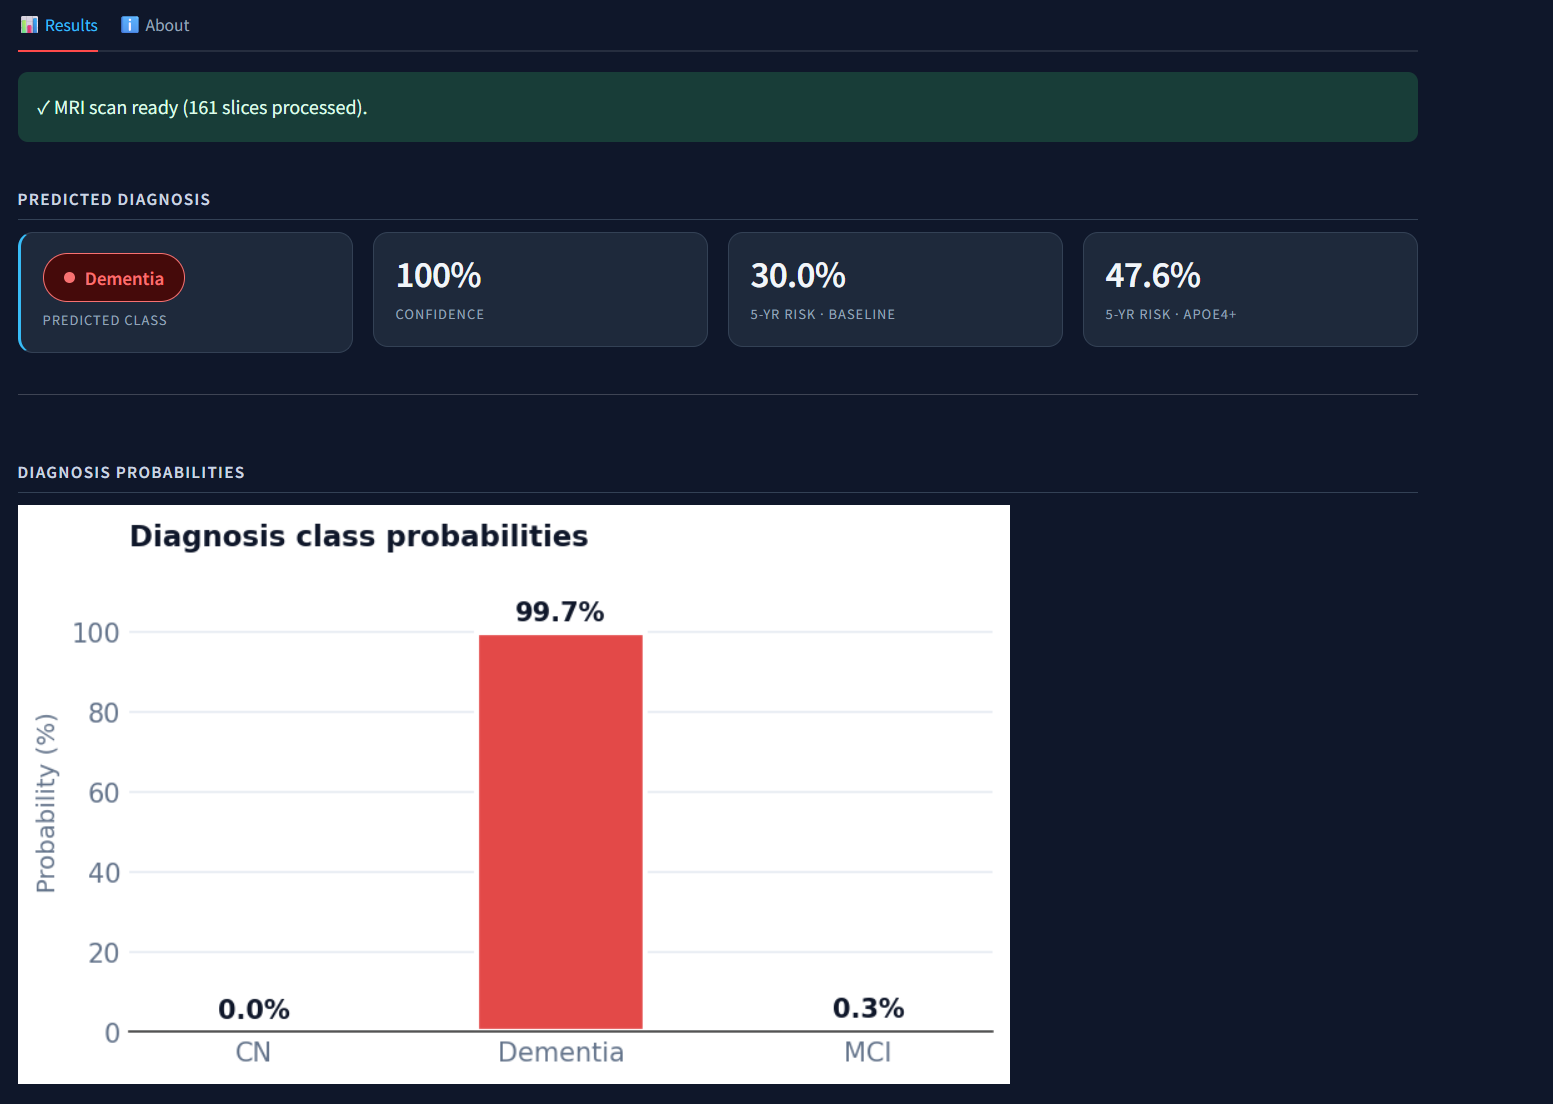
\includegraphics[width=0.95\columnwidth]{fig_dashboard_prediction.png}
\caption{Deployed dashboard, prediction output for the held-out verification patient.}
\label{fig:dashboard_prediction}
\end{figure}

\begin{figure}[t]
\centering
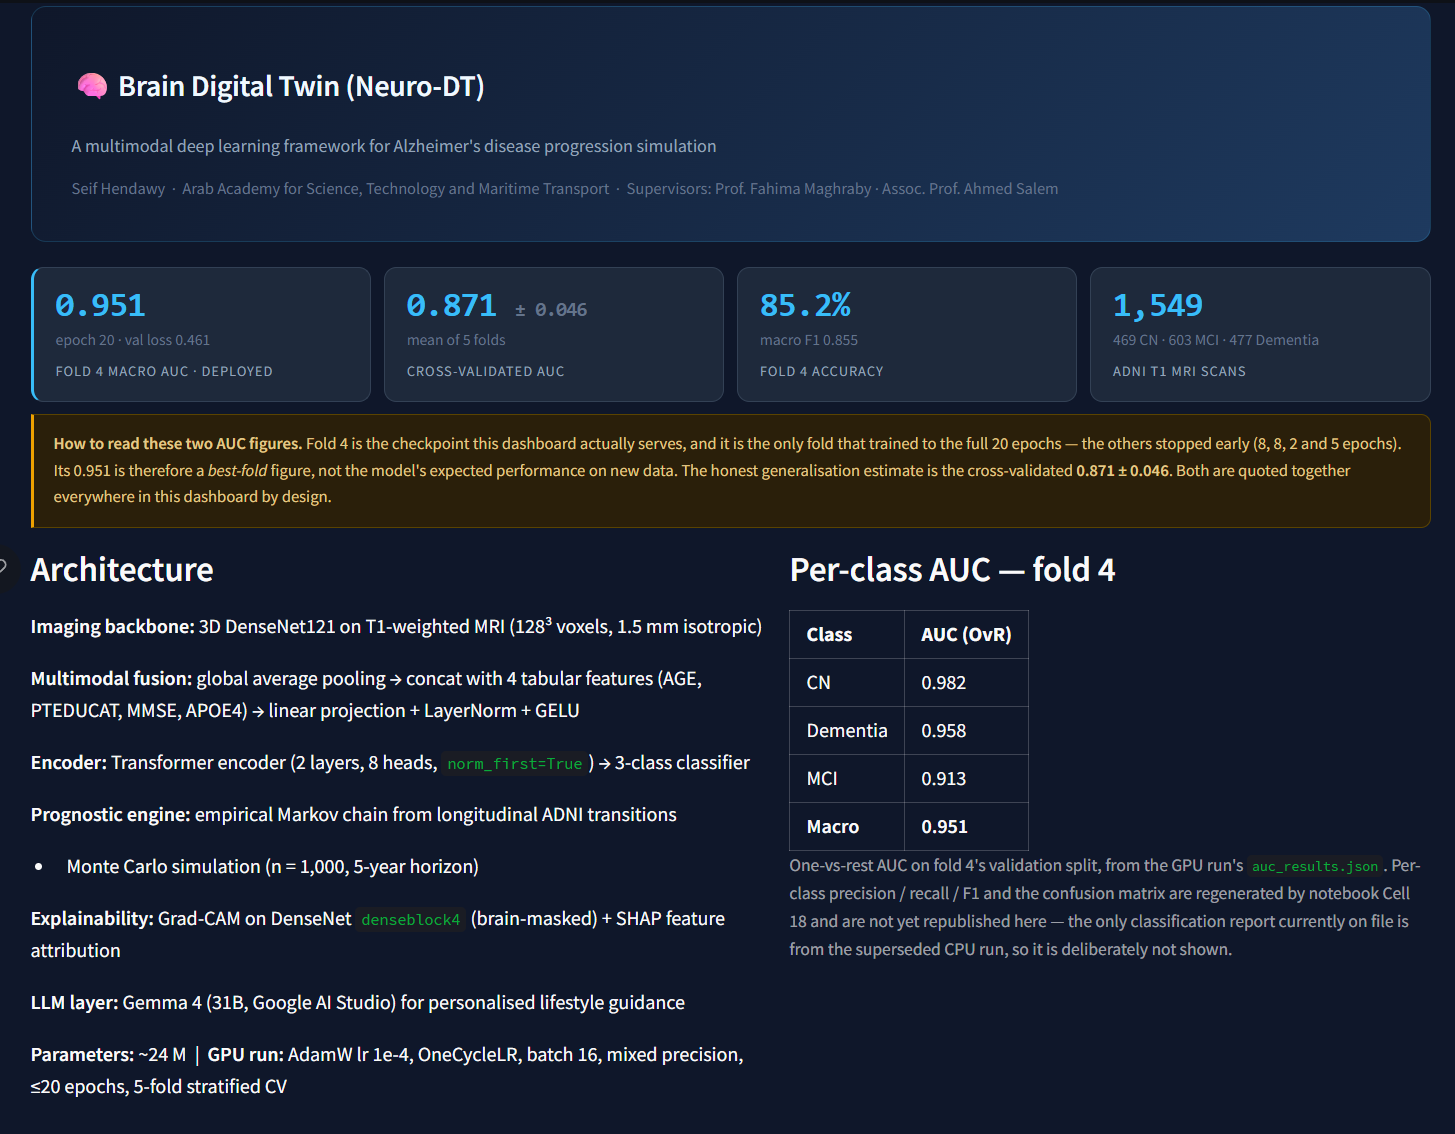
\includegraphics[width=0.85\columnwidth]{fig_dashboard_about.png}
\caption{Deployed dashboard, ``About'' / model-information panel.}
\label{fig:dashboard_about}
\end{figure}

\begin{figure}[t]
\centering
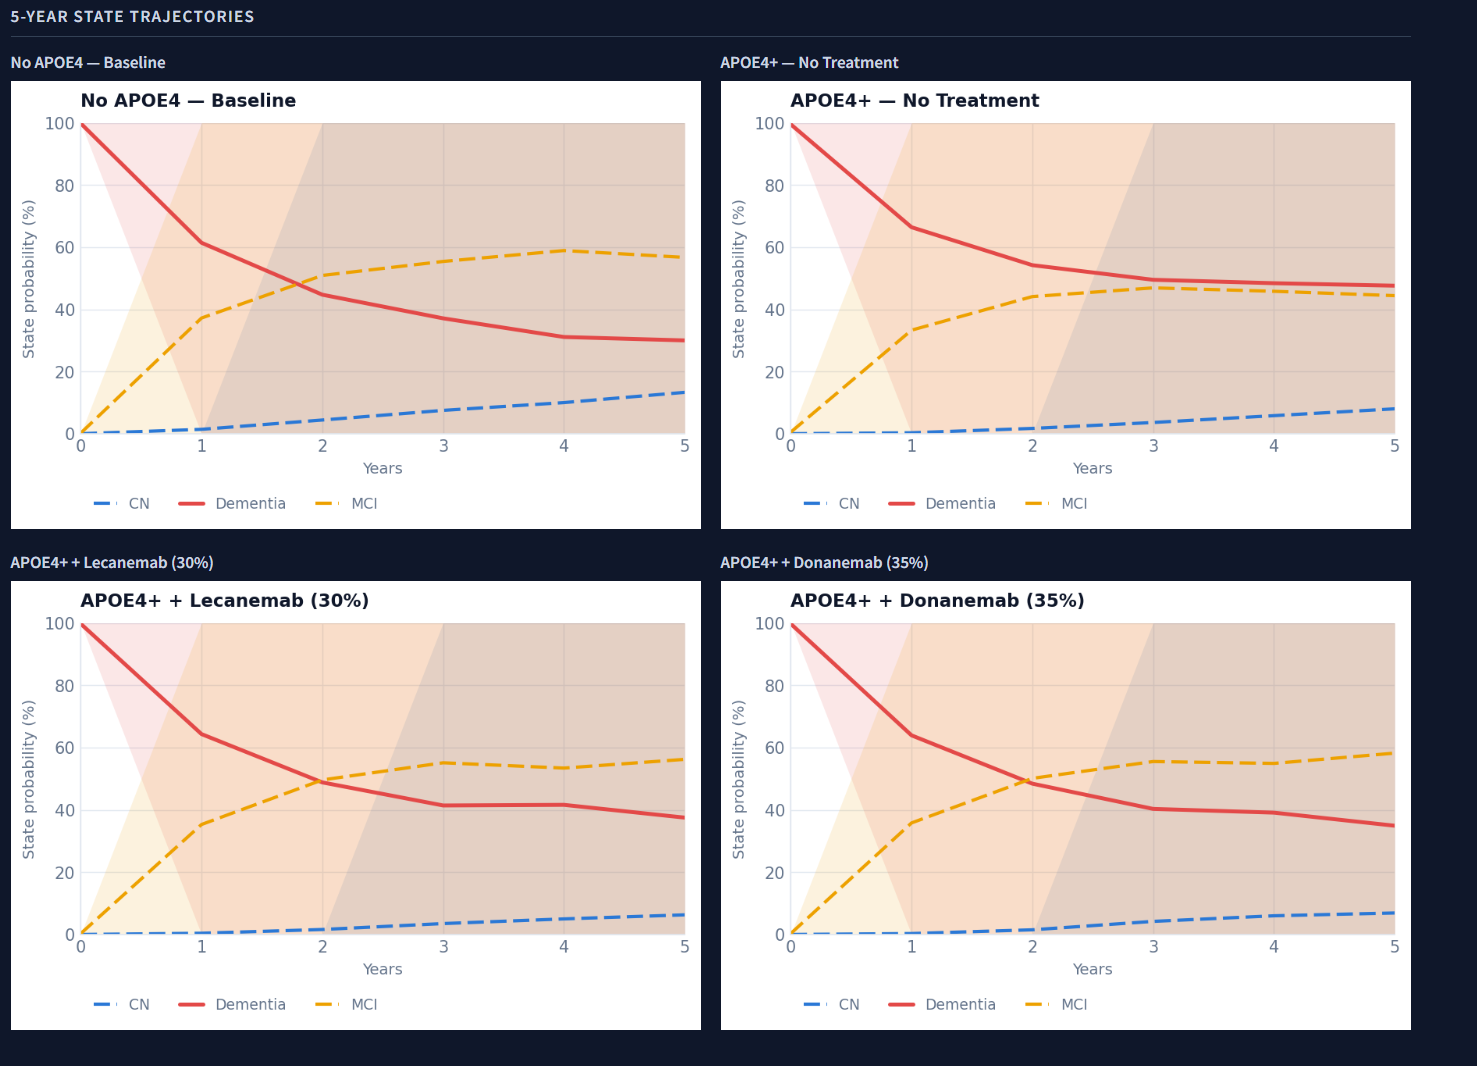
\includegraphics[width=0.95\columnwidth]{fig_dashboard_trajectories_tab.png}
\caption{Deployed dashboard, 5-year state-trajectories panel, four intervention scenarios for a single patient.}
\label{fig:dashboard_trajectories_tab}
\end{figure}

\begin{figure}[t]
\centering
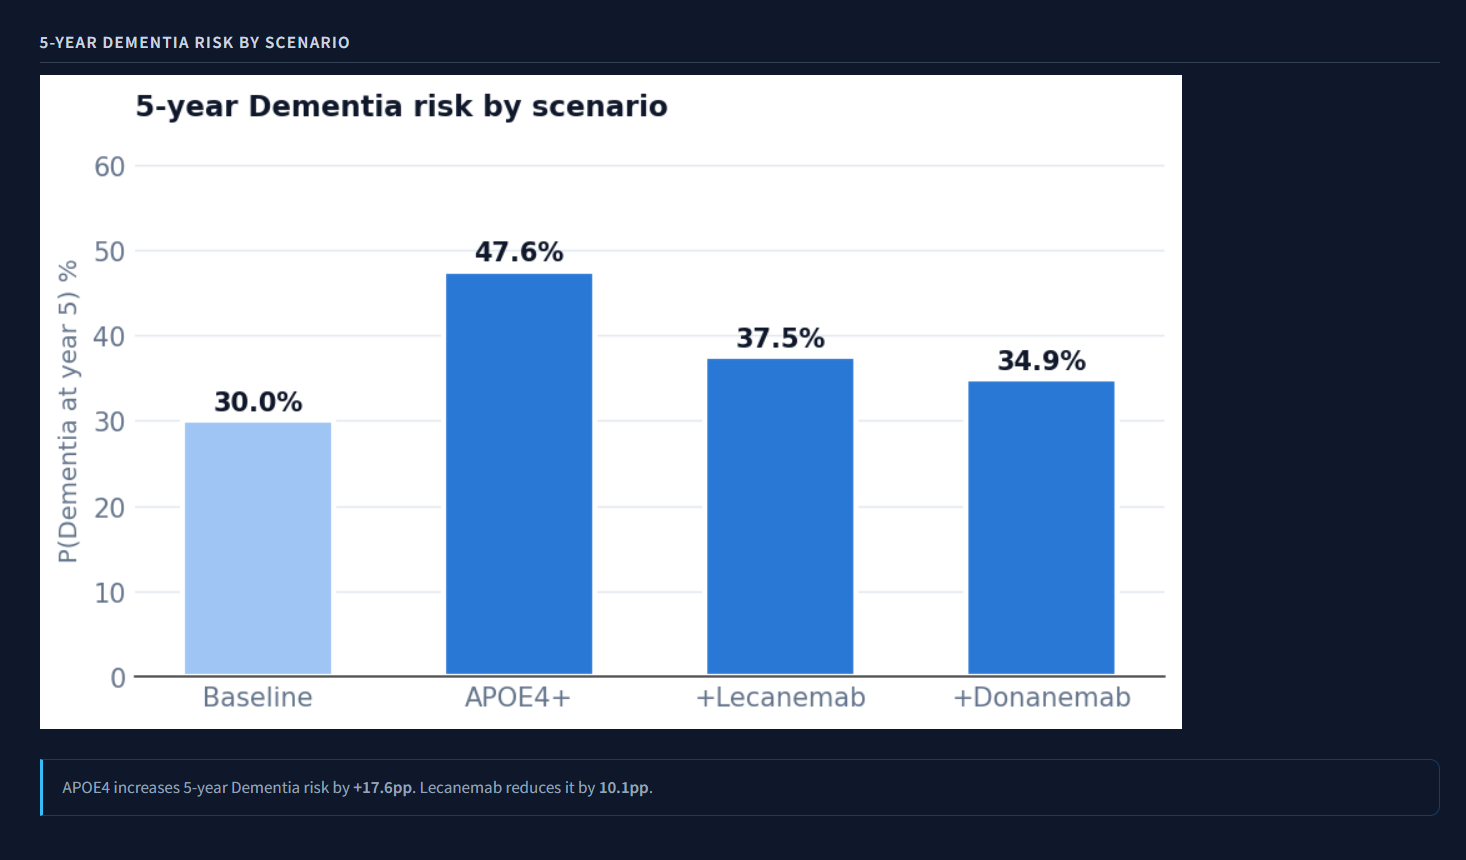
\includegraphics[width=0.9\columnwidth]{fig_dashboard_risk_factor.png}
\caption{Deployed dashboard, 5-year dementia risk-factor chart.}
\label{fig:dashboard_risk_factor}
\end{figure}

\begin{figure}[t]
\centering
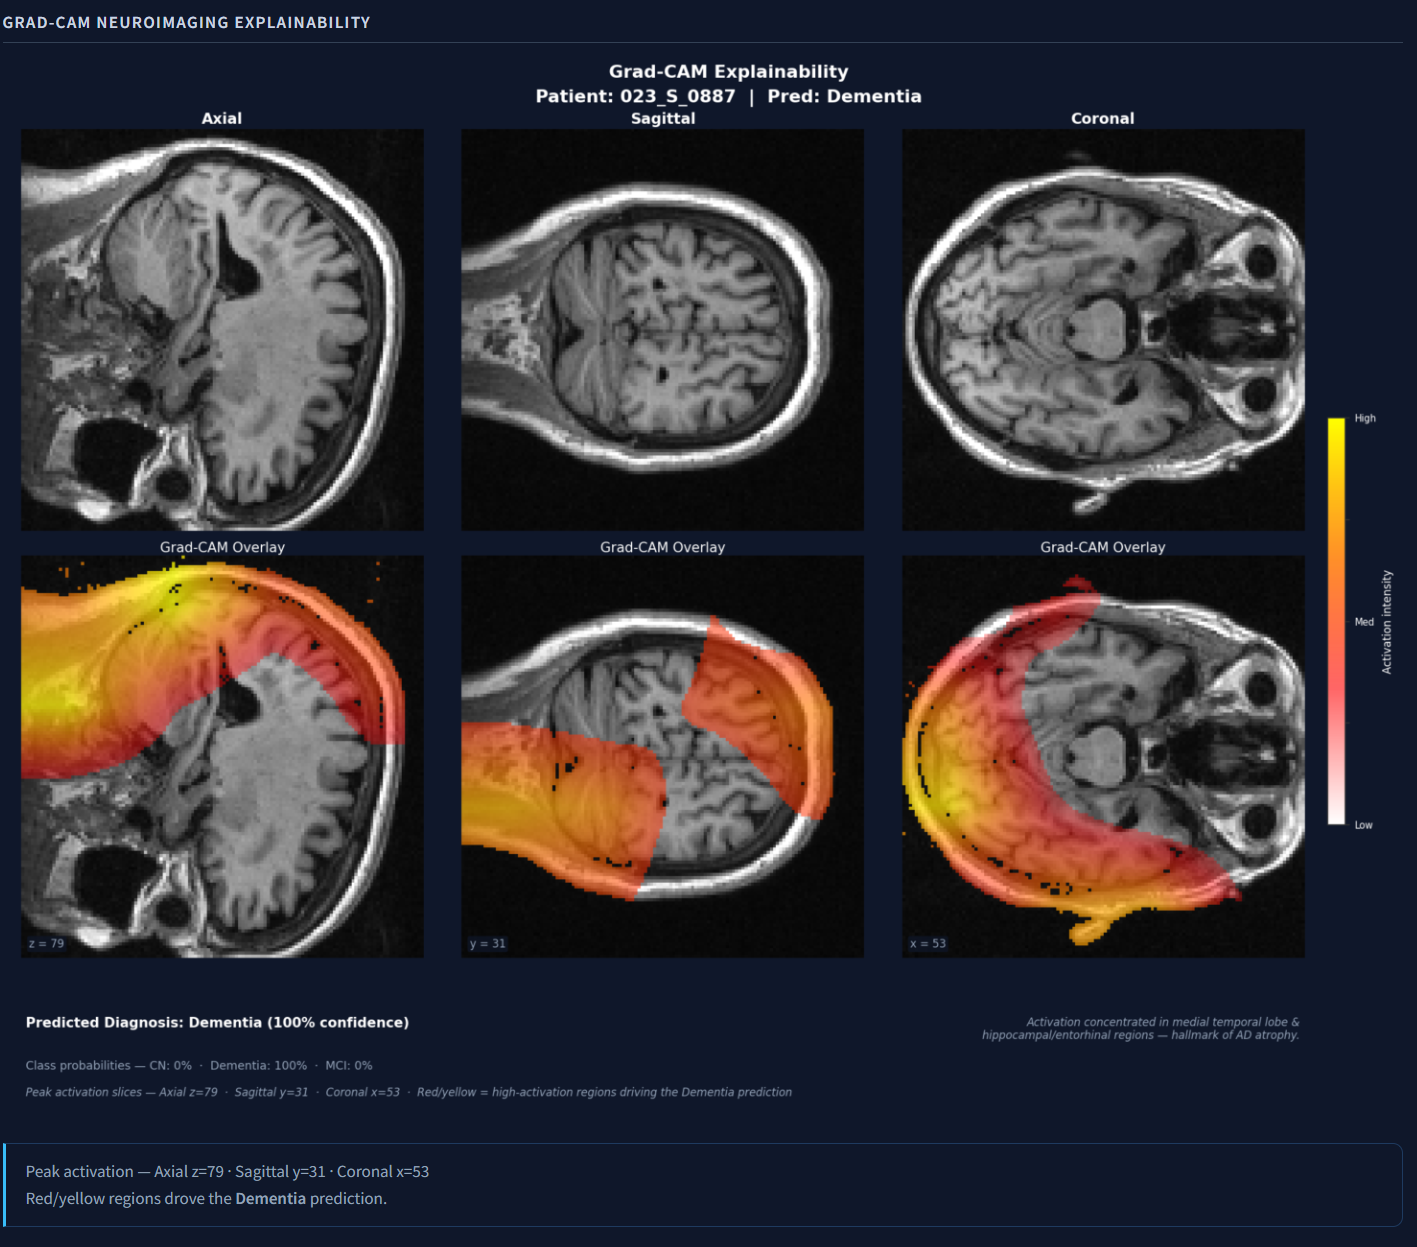
\includegraphics[width=0.85\columnwidth]{fig_dashboard_gradcam_demo.png}
\caption{Deployed dashboard, Grad-CAM explainability panel, live-generated overlay for Patient 023\_S\_0887.}
\label{fig:dashboard_gradcam_demo}
\end{figure}

\begin{figure}[t]
\centering
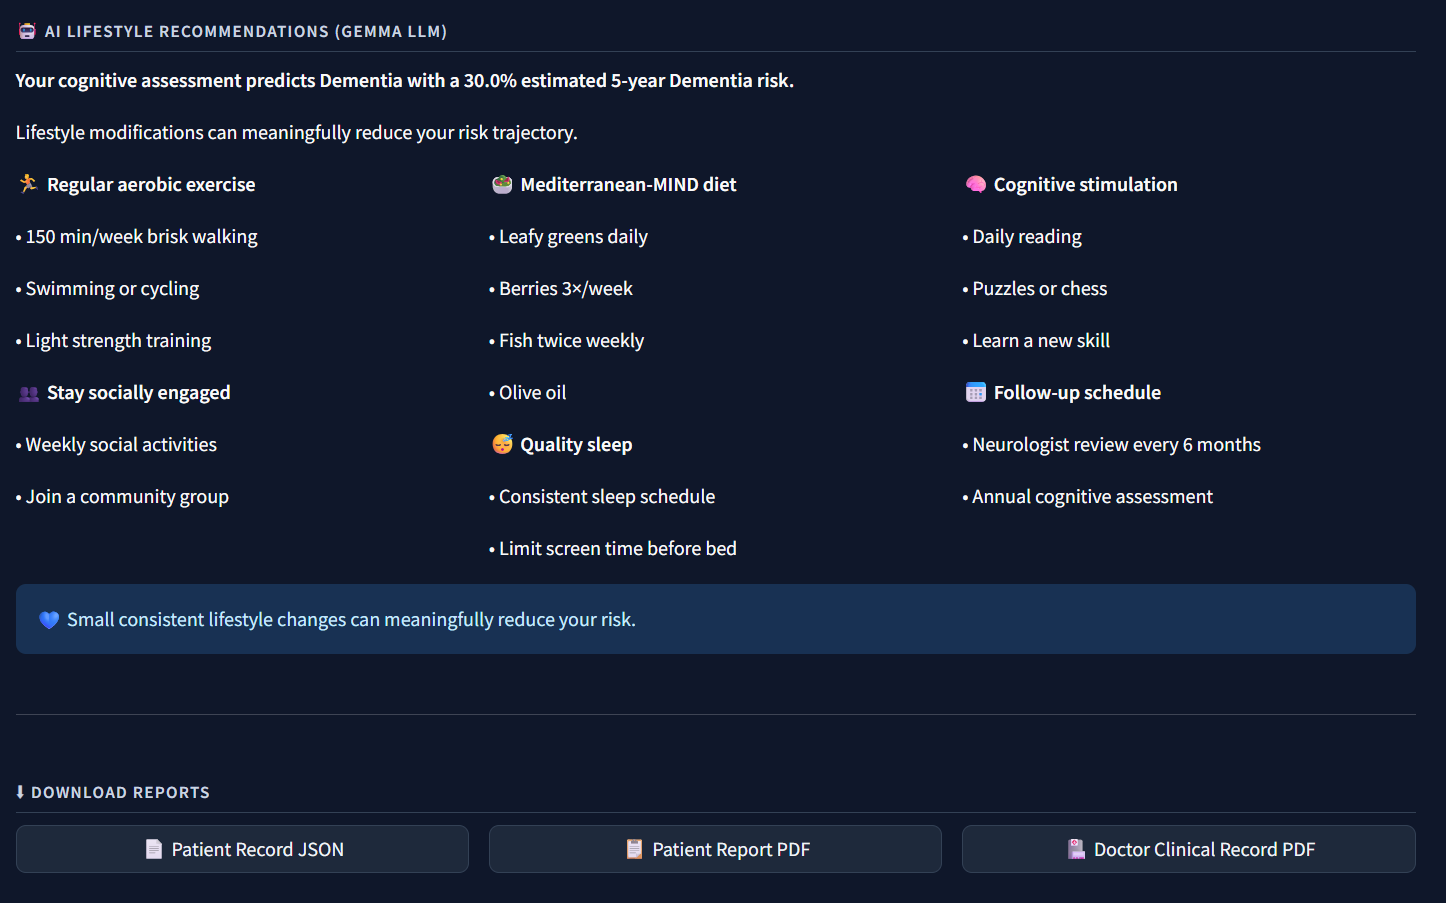
\includegraphics[width=0.95\columnwidth]{fig_dashboard_lifestyle.png}
\caption{Deployed dashboard, AI-generated lifestyle-recommendation panel.}
\label{fig:dashboard_lifestyle}
\end{figure}

\section{Impact}\label{sec4}

The Neuro-DT Dashboard turns a validated but code-only research pipeline into a tool a clinician or researcher can operate directly: selecting a patient, reading a diagnosis and its confidence, inspecting the anatomical and clinical basis for that diagnosis, and comparing simulated five-year outcomes under genetic-risk and pharmacological-intervention scenarios, all from one interface. This is the layer that a diagnostic classifier or a progression-simulation script alone does not provide: translating model output into something a non-programmer can read, question, and act on.

The three integration-stage defects documented in Section~\ref{sec2_1} are reported because none of them were visible from within the original training and evaluation environment; each one only surfaced once the same checkpoint and simulation code were run behind a persistent, request-driven web service rather than a one-shot script. The checkpoint-loading and label-mapping defects are specific instances of a general risk, that a model artifact's loading and metadata contract can silently drift between the environment it was trained in and the environment it is served from, and the silent-failure mode is a specific instance of a general risk in any multimodal clinical tool, that a missing input modality must be surfaced to the user rather than silently substituted and presented as if the prediction were unaffected. Documenting these as a software description, rather than only as a line item in a results table, is intended to make them reusable lessons for other groups deploying a research classifier or simulation model behind a clinical-facing interface.

The dashboard's architecture, a frozen checkpoint and transition matrices served behind a stateless Streamlit application with live explainability and simulation, is not specific to Alzheimer's Disease or to this particular classifier; the same pattern applies to any Digital Twin-style clinical tool that pairs a trained diagnostic model with a probabilistic progression simulator and needs to expose both, together with an explanation, to a non-technical user.

\section{Conclusions}\label{sec5}

The Neuro-DT Dashboard packages a trained hybrid 3D CNN-Transformer Alzheimer's classifier and an APOE4-stratified Markov progression model into a single Streamlit application, deployed to Azure App Service, that delivers a diagnosis, its live SHAP and Grad-CAM explanation, and a Monte Carlo what-if simulation under genetic-risk and pharmacological-intervention scenarios from one interface. The deployed application was validated against a genuine held-out patient record, and three integration-stage defects, undetectable from within the original research environment, were identified, fixed, and documented as reusable lessons for deploying similar clinical Digital Twin tools. Future work includes replacing the current 2D multi-planar Grad-CAM overlays with an interactive volumetric 3D visualization, and integrating per-patient medication history so that the intervention simulation reflects a patient's actual treatment record rather than a literature-derived uniform effect size \cite{bib_bdt}.

\section*{Declaration of Generative AI and AI-assisted technologies in the writing process}

During the preparation of this work the author(s) used Claude (Anthropic) to assist with drafting, editing, and restructuring portions of this manuscript's text. After using this tool, the author(s) reviewed and edited the content as needed and take full responsibility for the content of the published article and the accompanying software.

\section*{CRediT authorship contribution statement}

\textbf{Seif Hendawy:} Software, Writing -- original draft, Writing -- review \& editing, Visualization, Methodology, Conceptualization. \textbf{Fahima Maghraby:} Supervision, Writing -- review \& editing, Methodology. \textbf{Ahmed Salem:} Supervision, Writing -- review \& editing, Methodology.

\section*{Declaration of competing interest}

The authors declare that they have no known competing financial interests or personal relationships that could have appeared to influence the work reported in this paper.

\section*{Acknowledgements}

The authors gratefully acknowledge the Arab Academy for Science, Technology and Maritime Transport (AASTMT), Sheraton Branch, Cairo, Egypt, for providing the laboratory facilities used to develop and deploy the software described here. Data used in the development and validation of the underlying model were obtained from the Alzheimer's Disease Neuroimaging Initiative (ADNI) database.

\begin{thebibliography}{9}

\bibitem{bib_bdt} S. Hendawy, F. Maghraby, A. Salem, ``Brain Digital Twin (BDT): a hybrid 3D CNN-Transformer framework with Markov-based prognostic simulation for personalized Alzheimer's Disease progression modeling,'' \textit{manuscript in preparation}. \texttt{[UPDATE WITH FULL CITATION / DOI ONCE THE COMPANION PAPER IS SUBMITTED OR PUBLISHED]}

\bibitem{bib_shap} S. M. Lundberg, S.-I. Lee, ``A unified approach to interpreting model predictions,'' in \textit{Advances in Neural Information Processing Systems}, vol. 30, 2017, pp. 4765--4774.

\bibitem{bib_gradcam} R. R. Selvaraju, M. Cogswell, A. Das, R. Vedantam, D. Parikh, D. Batra, ``Grad-CAM: visual explanations from deep networks via gradient-based localization,'' in \textit{2017 IEEE International Conference on Computer Vision (ICCV)}, Venice, Italy, 2017, pp. 618--626. Available: \url{https://doi.org/10.1109/ICCV.2017.74}

\bibitem{bib_streamlit} Streamlit Inc., ``Streamlit: a faster way to build and share data apps,'' 2024. Available: \url{https://streamlit.io}

\bibitem{bib_lecanemab} C. H. van Dyck, S. Swanson, R. A. Aisen, et al., ``Lecanemab in early Alzheimer's Disease,'' \textit{The New England Journal of Medicine}, vol. 388, no. 1, pp. 9--21, 2023. Available: \url{https://doi.org/10.1056/NEJMoa2212948}

\bibitem{bib_dt_precision} K. P. Venkatesh, M. M. Raza, J. C. Kvedar, ``Health digital twins as tools for precision medicine: considerations for computation, implementation, and regulation,'' \textit{npj Digital Medicine}, vol. 5, 150, 2022. Available: \url{https://doi.org/10.1038/s41746-022-00694-7}

\bibitem{bib_dt_modular} J. Gaebel, J. Keller, D. Schneider, A. Lindenmeyer, T. Neumuth, S. Franke, ``The Digital Twin: modular model-based approach to personalized medicine,'' \textit{Current Directions in Biomedical Engineering}, vol. 7, no. 2, pp. 223--226, 2021. Available: \url{https://doi.org/10.1515/cdbme-2021-2057}

\bibitem{bib_dt_cardio} G. Coorey, G. A. Figtree, D. F. Fletcher, et al., ``The health digital twin to tackle cardiovascular disease: a review of an emerging interdisciplinary field,'' \textit{npj Digital Medicine}, vol. 5, no. 126, 2022. Available: \url{https://doi.org/10.1038/s41746-022-00640-7}

\bibitem{bib_qiu} S. Qiu, P. S. Joshi, M. I. Miller, et al., ``Development and validation of an interpretable deep learning framework for Alzheimer's disease classification,'' \textit{Brain}, vol. 143, no. 6, pp. 1920--1933, 2020. Available: \url{https://doi.org/10.1093/brain/awaa137}

\bibitem{bib_axial} G. Lozupone, A. Bria, F. Fontanella, F. J. A. Meijer, C. De Stefano, ``AXIAL: attention-based eXplainability for interpretable Alzheimer's localized diagnosis using 2D CNNs on 3D MRI brain scans,'' \textit{arXiv preprint arXiv:2407.02418}, 2024. Available: \url{https://doi.org/10.48550/arXiv.2407.02418}

\end{thebibliography}

\end{document}
